\documentclass[12pt]{article}

\usepackage{amsmath,amsthm,amsfonts,amssymb,amsxtra}
\usepackage{pgf,tikz}
\usetikzlibrary{arrows}
\renewcommand{\theenumi}{(\alph{enumi})} 
\renewcommand{\labelenumi}{\theenumi}

\pagestyle{empty}
\setlength{\textwidth}{7in}
\setlength{\oddsidemargin}{-0.5in}
\setlength{\topmargin}{-1.0in}
\setlength{\textheight}{9.5in}

\newtheorem{problem}{Problem}

\begin{document}

\noindent{\large\bf MATH 122}\hfill{\large\bf Third Midterm.}\hfill{\large\bf
  Spring 2012}\hfill{\large\bf Page 1/5}\hrule

\bigskip
\begin{center}
  \begin{tabular}{|ll|}
    \hline & \cr
    {\bf Name: } & \makebox[12cm]{\hrulefill}\cr & \cr
    {\bf 4-digit code:} & \makebox[12cm]{\hrulefill}\cr & \cr
    \hline
  \end{tabular}
\end{center}
\begin{itemize}
\item Write your name and the last 4 digits of your SSN in the space provided above.
\item The test has five (5) pages, including this one.
\item For multiple-choice questions, circle the answer you select.  On
  the other problems, you should enter your answer in the box(es)
  provided. 
\item Show sufficient work to justify all answers unless otherwise
  stated in the problem.  Correct answers with inconsistent work may
  not be given credit. 
\item Credit for each problem is given at the right of each problem
  number. 
\item No books or notes may be used on this test.  Calculators are
  allowed, provided they don't have a computer algebra system.
\end{itemize}
\hrule

\begin{center}
  \begin{tabular}{|c|c|c|}
    \hline
    &&\cr
    {\large\bf Page} & {\large\bf Max} & {\large\bf Points} \cr
    &&\cr
    \hline
    &&\cr
    {\Large 2} & \Large 30 & \cr
    &&\cr
    \hline
    &&\cr
    {\Large 3} & \Large 30 & \cr
    &&\cr
    \hline
    &&\cr
    {\Large 4} & \Large 20 & \cr
    &&\cr
    \hline
    &&\cr
    {\Large 5} & \Large 20 & \cr
    &&\cr
    \hline\hline
    &&\cr
    {\large\bf Total} & \Large 100 & \cr
    &&\cr
    \hline
  \end{tabular}
\end{center}
\newpage

%%%%%%%%%%%%%%%%%%%%%%%%%%%%%%%%%%%%% Page 2
\noindent{\large\bf MATH 122}\hfill{\large\bf Third Midterm.}\hfill{\large\bf
  Spring 2012}\hfill{\large\bf Page 2/5}\hrule

\bigskip
{\problem[10 pts] \em Find the derivative of the function
  $y=7e^{8t+1}$.}
\vspace{4.5cm}
\begin{flushright}
  \begin{tikzpicture}
    \draw (0cm,-0.2cm) rectangle (5cm,1.2cm);
  \end{tikzpicture}
\end{flushright}
\hrule
{\problem[10 pts] \em Find the derivative of the function $y=6+\ln
  (3t+2)$.}
\vspace{4.5cm}
\begin{flushright}
  \begin{tikzpicture}
    \draw (0cm,-0.2cm) rectangle (5cm,1.2cm);
  \end{tikzpicture}
\end{flushright}

\hrule
{\problem[10 pts] \em If $f(x)=(3x+6)(8x-3)$, find $f'(x)$ and
  $f''(x)$.}
\vspace{3cm}
\begin{flushright}
  \begin{tikzpicture}
    \draw (0cm,-0.2cm) rectangle (5cm,1.2cm);
    \draw (0cm,1.8cm) rectangle (5cm,3.2cm);
  \end{tikzpicture}
\end{flushright}
\newpage

%%%%%%%%%%%%%%%%%%%%%%%%%%%%%%%%%%%%% Page 3
\noindent{\large\bf MATH 122}\hfill{\large\bf Third Midterm.}\hfill{\large\bf
  Spring 2012}\hfill{\large\bf Page 3/5}\hrule

\bigskip
{\problem[10 pts] \em Find the derivative of the function
  $f(x)=8xe^x$.}
\vspace{4.5cm}
\begin{flushright}
  \begin{tikzpicture}
    \draw (0cm,-0.2cm) rectangle (5cm,1.2cm);
  \end{tikzpicture}
\end{flushright}
\hrule
{\problem[10 pts] \em  Find the derivative of $z=\dfrac{9-t}{9+t}$,}
\vspace{4.5cm}
\begin{flushright}
  \begin{tikzpicture}
    \draw (0cm,-0.2cm) rectangle (5cm,1.2cm);
  \end{tikzpicture}
\end{flushright}
\hrule
{\problem[10 pts] \em The figure below is a graph of $f'$.  Find the
  $x$--values that are critical points of the function $f$ itself.
  Are they local maxima, local minima, or neither?}

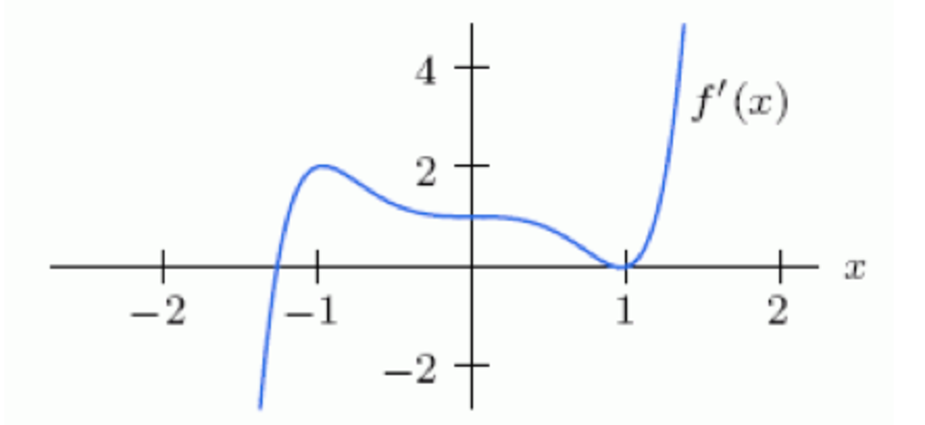
\includegraphics[width=8cm]{derivative.pdf}
\begin{flushright}
  \begin{tikzpicture}
    \draw (0cm,-0.2cm) rectangle (5cm,1.2cm);
    \draw (0cm, 1.8cm) rectangle (5cm,3.2cm);
  \end{tikzpicture}
\end{flushright}
\newpage

%%%%%%%%%%%%%%%%%%%%%%%%%%%%%%%%%%%%% Page 4
\noindent{\large\bf MATH 122}\hfill{\large\bf Third Midterm.}\hfill{\large\bf
  Spring 2012}\hfill{\large\bf Page 4/5}\hrule

\bigskip
{\problem[10 pts] \em Find an antiderivative $F(x)$ of
  $f(x)=9x^4+22x+2$ that satisfies $F(0)=7$.}
\vspace{6cm}
\begin{flushright}
  \begin{tikzpicture}
    \draw (0cm,-0.2cm) rectangle (5cm,1.2cm);
  \end{tikzpicture}
\end{flushright}
\hrule
{\problem[10 pts] \em Let $C(q)$ represent the cost, $R(q)$ the
  revenue, and $\Pi(q)$ the total profit, in dollars, of producing $q$
items.}
\begin{enumerate}
\item If $C'(50)=75$ and $R'(50)=82$, approximately how much profit is
  earned by the $51^{st}$ item?
\vspace{3cm}
\item If $C'(90)=69$ and $R'(90)=63$, approximately how much profit is
  earned by the $91^{st}$ item?
\vspace{3cm}
\item If $\Pi(q)$ is a maximum when $q=78$, how do you think $C'(78)$
  and $R'(78)$ compare?
\end{enumerate}
\newpage

%%%%%%%%%%%%%%%%%%%%%%%%%%%%%%%%%%%%% Page 5
\noindent{\large\bf MATH 122}\hfill{\large\bf Third Midterm.}\hfill{\large\bf
  Spring 2012}\hfill{\large\bf Page 5/5}\hrule

\bigskip
{\problem[10 pts] \em Find the integral $\displaystyle{\int 60e^{2x}\,
    dx}$} 
\vspace{8cm}
\begin{flushright}
  \begin{tikzpicture}
    \draw (0cm,-0.2cm) rectangle (5cm,1.2cm);
  \end{tikzpicture}
\end{flushright}
{\problem[10 pts] \em Find the integral $\displaystyle{\int
   \frac{x}{3x^2+9}\, dx}$.}
\vspace{8cm}
\begin{flushright}
  \begin{tikzpicture}
    \draw (0cm,-0.2cm) rectangle (5cm,1.2cm);
  \end{tikzpicture}
\end{flushright}
\end{document}
